\documentclass[12pt]{scrartcl}
 \usepackage{fancyhdr, graphicx}
 \usepackage[utf8]{inputenc} 
 \usepackage[german]{babel}
 \usepackage[scaled=0.92]{helvet}
 \usepackage{enumitem}
 \usepackage{parskip}
 \usepackage[utf8]{inputenc}
 \usepackage{listingsutf8}
 \usepackage{lastpage} % for getting last page number
 \renewcommand{\familydefault}{\sfdefault}
 
 % Code listenings
\usepackage{color}
\usepackage{xcolor}
\usepackage{caption}
\DeclareCaptionFont{white}{\color{white}}
\DeclareCaptionFormat{listing}{\colorbox{gray}{\parbox{\textwidth}{#1#2#3}}}
\captionsetup[lstlisting]{format=listing,labelfont=white,textfont=white}
\lstset{literate=%
    {Ö}{{\"O}}1
    {Ä}{{\"A}}1
    {Ü}{{\"U}}1
    {ß}{{\ss}}1
    {ü}{{\"u}}1
    {ä}{{\"a}}1
    {ö}{{\"o}}1
    {á}{{\'a}}1
    {í}{{\'i}}1
    {é}{{\'e}}1
    {ý}{{\'y}}1
    {ú}{{\'u}}1
    {ó}{{\'o}}1
    {é}{{\'{e}}}1
    {è}{{\`{e}}}1
    {È}{{\`{E}}}1
    {ê}{{\^{e}}}1
    {ë}{{\¨{e}}}1
    {É}{{\'{E}}}1
    {Ê}{{\^{E}}}1
    {û}{{\^{u}}}1
    {ù}{{\`{u}}}1
    {â}{{\^{a}}}1
    {à}{{\`{a}}}1
    {á}{{\'{a}}}1
    {ã}{{\~{a}}}1
    {Á}{{\'{A}}}1
    {Â}{{\^{A}}}1
    {Ã}{{\~{A}}}1
    {ç}{{\c{c}}}1
    {Ç}{{\c{C}}}1
    {õ}{{\~{o}}}1
    {ó}{{\'{o}}}1
    {ô}{{\^{o}}}1
    {Õ}{{\~{O}}}1
    {Ó}{{\'{O}}}1
    {Ô}{{\^{O}}}1
    {î}{{\^{i}}}1
    {Î}{{\^{I}}}1
    {í}{{\'{i}}}1
    {Í}{{\~{Í}}}1
    {ě}{{\v{e}}}1
    {š}{{\v{s}}}1
    {č}{{\v{c}}}1
    {ř}{{\v{r}}}1
    {ž}{{\v{z}}}1
    {ď}{{\v{d}}}1
    {ť}{{\v{t}}}1
    {ň}{{\v{n}}}1                
    {ů}{{\r{u}}}1
    {Á}{{\'A}}1
    {Í}{{\'I}}1
    {É}{{\'E}}1
    {Ý}{{\'Y}}1
    {Ú}{{\'U}}1
    {Ó}{{\'O}}1
    {Ě}{{\v{E}}}1
    {Š}{{\v{S}}}1
    {Č}{{\v{C}}}1
    {Ř}{{\v{R}}}1
    {Ž}{{\v{Z}}}1
    {Ď}{{\v{D}}}1
    {Ť}{{\v{T}}}1
    {Ň}{{\v{N}}}1                
    {Ů}{{\r{U}}}1
    {~}{{\textasciitilde}}1
}
\lstdefinestyle{SQLStyle}{
morekeywords={CREATE TABLE IF NOT EXISTS, COLLATE, NOT NULL, ENGINE, PRIMARY KEY,DEFAULT CHARSET},
 language=sql,
 basicstyle=\footnotesize\ttfamily, % Standardschrift
 numbers=left, % Ort der Zeilennummern
 numberstyle=\tiny, % Stil der Zeilennummern
 stepnumber=5, % Abstand zwischen den Zeilennummern
 numbersep=5pt, % Abstand der Nummern zum Text
 tabsize=2, % Groesse von Tabs
 extendedchars=true, %
 breaklines=true, % Zeilen werden Umgebrochen
 frame=b,
 %commentstyle=\itshape\color{LightLime}, Was isch das? O_o
 %keywordstyle=\bfseries\color{DarkPurple}, und das O_o
 basicstyle=\footnotesize\ttfamily,
 stringstyle=\color[RGB]{42,0,255}\ttfamily, % Farbe der String
 keywordstyle=\color[RGB]{127,0,85}\ttfamily, % Farbe der Keywords
 commentstyle=\color[RGB]{63,127,95}\ttfamily, % Farbe des Kommentars
 showspaces=false, % Leerzeichen anzeigen ?
 showtabs=false, % Tabs anzeigen ?
 xleftmargin=17pt,
 framexleftmargin=17pt,
 framexrightmargin=5pt,
 framexbottommargin=4pt,
 showstringspaces=false % Leerzeichen in Strings anzeigen ?
}

\lstdefinestyle{JavaStyle}{
 language=java,
 basicstyle=\footnotesize\ttfamily, % Standardschrift
 numbers=left, % Ort der Zeilennummern
 numberstyle=\tiny, % Stil der Zeilennummern
 stepnumber=5, % Abstand zwischen den Zeilennummern
 numbersep=5pt, % Abstand der Nummern zum Text
 tabsize=2, % Groesse von Tabs
 extendedchars=true, %
 breaklines=true, % Zeilen werden Umgebrochen
 frame=b,
 %commentstyle=\itshape\color{LightLime}, Was isch das? O_o
 %keywordstyle=\bfseries\color{DarkPurple}, und das O_o
 basicstyle=\footnotesize\ttfamily,
 stringstyle=\color[RGB]{42,0,255}\ttfamily, % Farbe der String
 keywordstyle=\color[RGB]{127,0,85}\ttfamily, % Farbe der Keywords
 commentstyle=\color[RGB]{63,127,95}\ttfamily, % Farbe des Kommentars
 showspaces=false, % Leerzeichen anzeigen ?
 showtabs=false, % Tabs anzeigen ?
 xleftmargin=17pt,
 framexleftmargin=17pt,
 framexrightmargin=5pt,
 framexbottommargin=4pt,
 showstringspaces=false % Leerzeichen in Strings anzeigen ?
}
 
 \captionsetup[lstlisting]{format=listing,labelfont=white,textfont=white}
 \fancypagestyle{firststyle}{ %Style of the first page
 \fancyhf{}
 \fancyheadoffset[L]{0.6cm}
 \lhead{
 
\includegraphics[scale=0.8]{./fhnw_ht_e_10mm.jpg}}
 \renewcommand{\headrulewidth}{0pt}
 \lfoot{APSI Lab 2}
 \rfoot{Daniel Gürber, Stefan Eggenschwiler}
}

\fancypagestyle{documentstyle}{ %Style of the rest of the document
 \fancyhf{}
 \fancyheadoffset[L]{0.6cm}
\lhead{
 
\includegraphics[scale=0.8]{./fhnw_ht_e_10mm.jpg}}
 \renewcommand{\headrulewidth}{0pt}
 \lfoot{\thepage\ / 3 }
}

\pagestyle{firststyle} %different look of first page
 
\author{Stefan Eggenschwiler \& Daniel Gürber}
\title{ %Titel
Application Security
\\Lab 2
\vspace{0.2cm}
}

 \begin{document}
 \maketitle
 \thispagestyle{firststyle}
 \pagestyle{firststyle}
 \begin{abstract}
 \begin{center}
 \end{center}
 \vspace{0.5cm}
\hrulefill
\end{abstract}

 \pagestyle{documentstyle}
 \tableofcontents
 \pagebreak
\section{Aufgabenstellung}
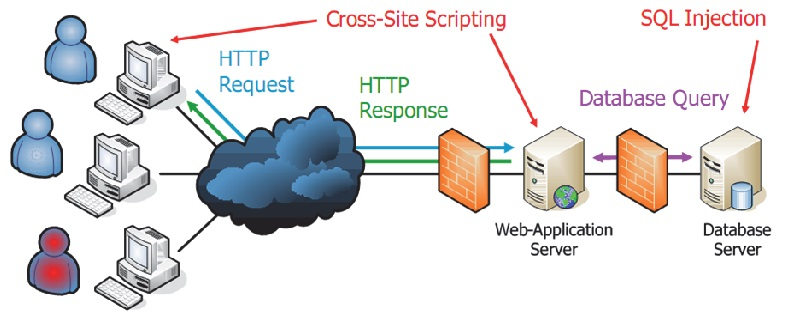
\includegraphics[scale=0.5]{./aufgabenstellung.jpg}

\section{Softwareaufbau}


\section{Datenbank}
\subsection{Aufbau}
\lstinputlisting[caption=Database Script,style=SQLStyle]{data_structure.sql}
\subsection{Sicherheit}

\section{Validierung}
Im folgenden gehen wir auf die Validierung der Inputdaten ein. Angegeben werden jeweils die Voraussetzungen aus der Aufgabenstellung und wie wir diese implementiert haben.

\subsection{Firmenname}
Nur Gross- und Klein-Buchstaben und Leerzeichen (max. 20).
\lstinputlisting[caption=Validierung Firmenname,style=JavaStyle]{firma.java}

\subsection{Strasse \& Strassennummer}
Gross- und Klein-Buchstaben, Zahlen, Punkt, Bindestrich, Leerzeichen.
\lstinputlisting[caption=Validierung Adresse,style=JavaStyle]{address.java}

\subsection{Postleitzahl}
Nur Zahlen, richtige PLZ für die Schweiz, nachkontrolliert mit einem Web-Dienst wie z. B.: http://www.postleitzahlen.ch.
\lstinputlisting[caption=Validierung PLZ,style=JavaStyle]{zip.java}

\subsection{Stadt}
Erlaubte Zeichen: Gross- und Klein-Buchstaben, Punkt, Bindestrich, Leerzeichen.
\lstinputlisting[caption=Validierung Stadt,style=JavaStyle]{town.java}

\subsection{E-Mail Adresse}
Sie senden aber erst, wenn Sie sicher sind, dass die
Email-Adresse auch existiert (no bouncing).
\lstinputlisting[caption=Validierung E-Mail,style=JavaStyle]{mail.java}

\subsection{Benutzername}
min. 4 Zeichen, max. 64 Zeichen; Erlaubte Zeichen:
Zahlen, Gross- und Klein-Buchstaben mit Umlauten, Punkte, Bindestriche, Unterstriche.

\subsection{Passwort}
min. 8 Zeichen, max. 64 Zeichen; Erlaubte Zeichen: Zahlen, Gross- und Klein-Buchstaben mit Umlauten, Punkten, Bindestrichen, Unterstrichen.
\lstinputlisting[caption=Validierung Passwort,style=JavaStyle]{password.java}

\section{Sicherheit}
\subsection{SQL-Injection \& Cross-site Scripting}


\subsection{Error Handling}


\subsection{Passwortspeicherung}


\section{SSL}

\end{document}